\chapter{Oide effect}
This part of the document addresses the radiation phenomena called Oide effect\cite{Oide}, which sets a limit on the beam size demagnification, specially important in linear colliders because of the strong focusing required in the Final Doublet before the Interation Point (IP).\par
First, a brief introduction to the beam size limit (Oide limit) is given, where adittional calculations have been derived to include this radiation phenomenon in the lattice design and optimization. The Oide effect is evaluated for the CLIC 3 TeV and CLIC 500 GeV parameters, leading to change the length of the first quadrupole before the IP, called QD0. It ends with a proposal to mitigate the impact of the strong focusing by adding correctors before and after the QD0, recovering part of the luminosity.\par
\section{Beam size limit}\label{Oideeffect}
The Oide effect is caused by the interaction of charged particles with the magnetic field from quadrupoles. Radiation in a focusing magnet, schematically represented as QD0 in Fig. (\ref{f:Oideeffect}), changes the energy of the particle and limits the focusing effect upstream the Interaction Point (IP). This imposes a limit on the minimum beam size specially relevant in the vertical plane.\par%For the horizontal direction, is mainly affected by radiation caused by the interaction of charged particles with the magnetic field from dipoles. %This report will be limited to sector dipoles or ``sbends''.\par
\begin{figure}[!hbt]
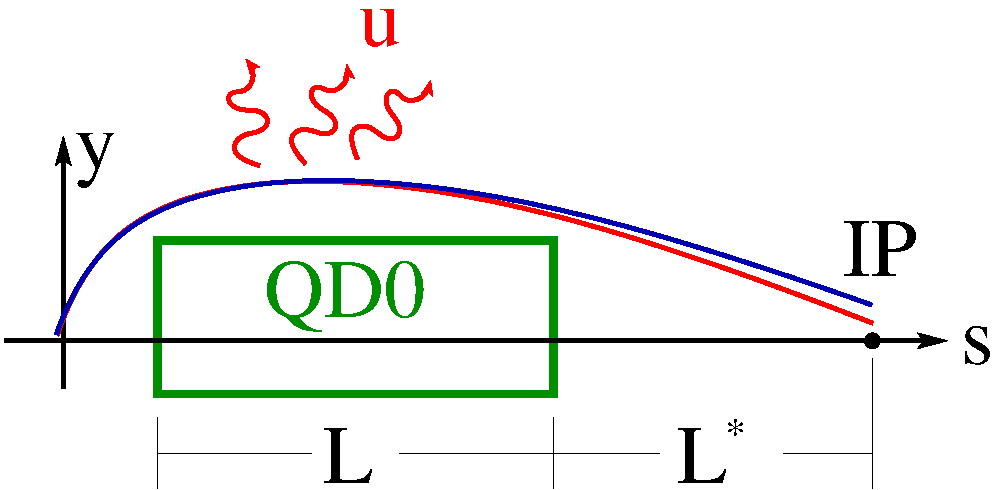
\includegraphics[scale=0.5]{Oide.pdf}
\centering
\caption{Designed particle trajectory in blue and the trajectory of a particle due to radiation in the quadrupole in red.}\label{f:Oideeffect}
\end{figure}
 The beam size growth due to radiation is added quadratically to the linear beam size $\sigma_0^2=\epsilon\beta$ where $\beta$ is optical beta function and $\epsilon$ is the emittance. Therefore, $ \sigma^2 = \sigma_0^2 + \sigma_{oide}^2$, and the beam size contribution is,
 \begin{equation}
  \sigma^2_{oide} = \frac{110}{3\sqrt{6\pi}}r_e\frac{\lambda_e}{2\pi}\gamma^5 F(\sqrt{k}L,\sqrt{k}L^*)\left(\frac{\epsilon}{\beta^*}\right)^{5/2}
  \label{Oideequ}
 \end{equation}
 where
 \begin{equation}
  F(\sqrt{k}L, \sqrt{k}L^*) = \int_0^{\sqrt{k}L}|\sin\phi+\sqrt{k}L^*\cos\phi|^3\left[\int_0^\phi(\sin\phi'+\sqrt{k}L^*\cos\phi')^2 d\phi'\right]^2d\phi
  \label{OideF}
 \end{equation}
  and $\lambda_e$ is the Compton wavelength of the electron, $r_e$ is the classical electron radius, $\gamma$ is the relativistic factor, $\epsilon$ is the geometrical beam emittance, $\beta^*$ is the Twiss parameter at the observation point (in this case, the IP), and $k$, $L$ and $L^*$ are the quadrupole gradient, the quadrupole length and the distance to the observation point measured from the closest magnet face.\par
  The double integral used to calculate $F$ has been solved with the goal to increase the computational calculation speed. It was included in MapClass2\cite{Mapclassorig,Mapclass,Mapclass2,githubMapClass2} to be used in lattice design and optimization, and can be found in Appendix \ref{c:primitiveF}.\par
   Although the total contribution to beam size depends on lattice and beam parameters, the minimum achievable beam size is given by
%the function $F$ is calculated only from quadrupole parameters. For this reason, $F$ will be used as figure of merit for a quadrupole.
\begin{equation}
 \sigma_{y \text{ min}} = \left(\frac{7}{5}\right)^\frac{1}{2}\left[\frac{275}{3\sqrt{6\pi}}r_e\frac{\lambda_e}{2\pi}F(\sqrt{K}L,\sqrt{K}L^*)\right]^\frac{1}{7}(\epsilon_{Ny})^\frac{5}{7}
\end{equation}
where $\epsilon_N=\gamma\epsilon$ is the normalized emittance, showing the independence from beam energy.\par
Beam size reduction is limited to change the value of $F$ by modifying the magnet parameters or to minimize the beam emittance. However, using the ILC 500 GeV \cite{ILCdes}, CLIC 500 GeV and CLIC 3 TeV \cite{CLICdes} parameters, it is possible to conclude from columns $\sigma_0$ and $\sigma_{oide}$ in Table (\ref{t:Sigmas}) that the contribution to beam size is only relevant for CLIC 3 TeV.\par
In addition, columns $\sigma$ and $\sigma_{min}$ in Table (\ref{t:Sigmas}) show that both CLIC designs are close to the minimum achievable beam size.\par
\begin{table}[!hbt]
\centering
{\scriptsize
\begin{tabular}{l||c|c|c||c|c|c|c|c||c|c}\hline\hline
Lattice &$\epsilon_N$& $\gamma$& $\sigma_0$&$k$&$L$&$L^*$& $F$ & $\sigma_{oide}$&$\sigma$&$\sigma_{min}$\\
 &(nm)&($10^3$)&(nm)&(m$^{-2}$)&(m)&(m)&&(nm) &(nm)&(nm)\\\hline
CLIC 3 TeV & 20 & 2935.0 & 0.70 & 0.116 & 2.73 &3.5&  4.086  & 0.85 & 1.10& 1.00 \\
CLIC 500 GeV & 25 & $\;\;$489.2 & 2.3 & 0.077 & 3.35 &4.3& 4.115 & 0.08 & 2.3 & 1.17\\
ILC  500 GeV & 40 & $\;\;$489.2 & 5.7 & 0.170 & 2.20 &4.3& 9.567 & 0.04 & 5.7 & 1.85\\\hline
\end{tabular}\caption{Vertical beam size and radiation beam size contribution for three lattices. $\epsilon_N$ is the normalized emittance, $\epsilon_N=\gamma\epsilon$.}\label{t:Sigmas}
}
\end{table}
\section{Mitigation on the beam size impact}
\subsection{QD0 length}
As shown in Sect. \ref{Oideeffect} the Oide beam size contribution depends on combination of beam and optics parameters. %Table \ref{tabSigmas} gives the results.
If none of the beam parameters is to be changed then $F$ can be used as a figure of merit of the optics as it is calculated only from $k$, $L$ and $l^*$. The target is to reduce it as much as possible and two energy cases are analyzed: 3 TeV ($l^*=3.5$ m) and 500 GeV ($l^*=4.3$ m).\par
Columns $\sigma_0$, $\sigma_{oide}$ and $F$ in Table \ref{t:Sigmas} show that CLIC 3 TeV and 500 GeV \cite{CLICdes,TomasCLIC} have larger contributions to beam size even having a lower $F$ value than ILC 500 GeV \cite{ILCdes}.\par
In order to evaluate the minimum possible $F$ for $L$ and $l^*$ given, the minimum $k$ required to get the particles focused is when the Twiss function $\alpha$ is zero just at the quadrupole opposite face to the IP.\par
Fig. \ref{fig-3TeV:a}  shows the ratio squared between the beam size contribution due to Oide effect and the linear beam size for three cases: when $k$ is the minimum required to get particles focused (to get $\alpha_y=0$ at QD0 opposite side to the IP), when $k$ is calculated as thin lens ($k=\frac{1}{Ll^*}$), and the current QD0 status. Fig. \ref{fig-3TeV:b} shows the $k$ values for the previous mentioned cases.\par
The Oide contribution to beam size is of the same order of the linear beam size. It might be possible to reduce it by doubling the current quad length and using a less conservative $k$ between the minimum required focusing and the thin lens approximation. This points to increase the lattice length as this change reduces the tolerance to variations of $\alpha$ at the quadrupole input.\par
Quad lengths larger than 10 m do not lead to further improvements with the current parameters.\par

\begin{figure}[!htb]
\centering
\hspace*{-0.6cm}
\begin{subfigure}{0.45\textwidth}
\centering
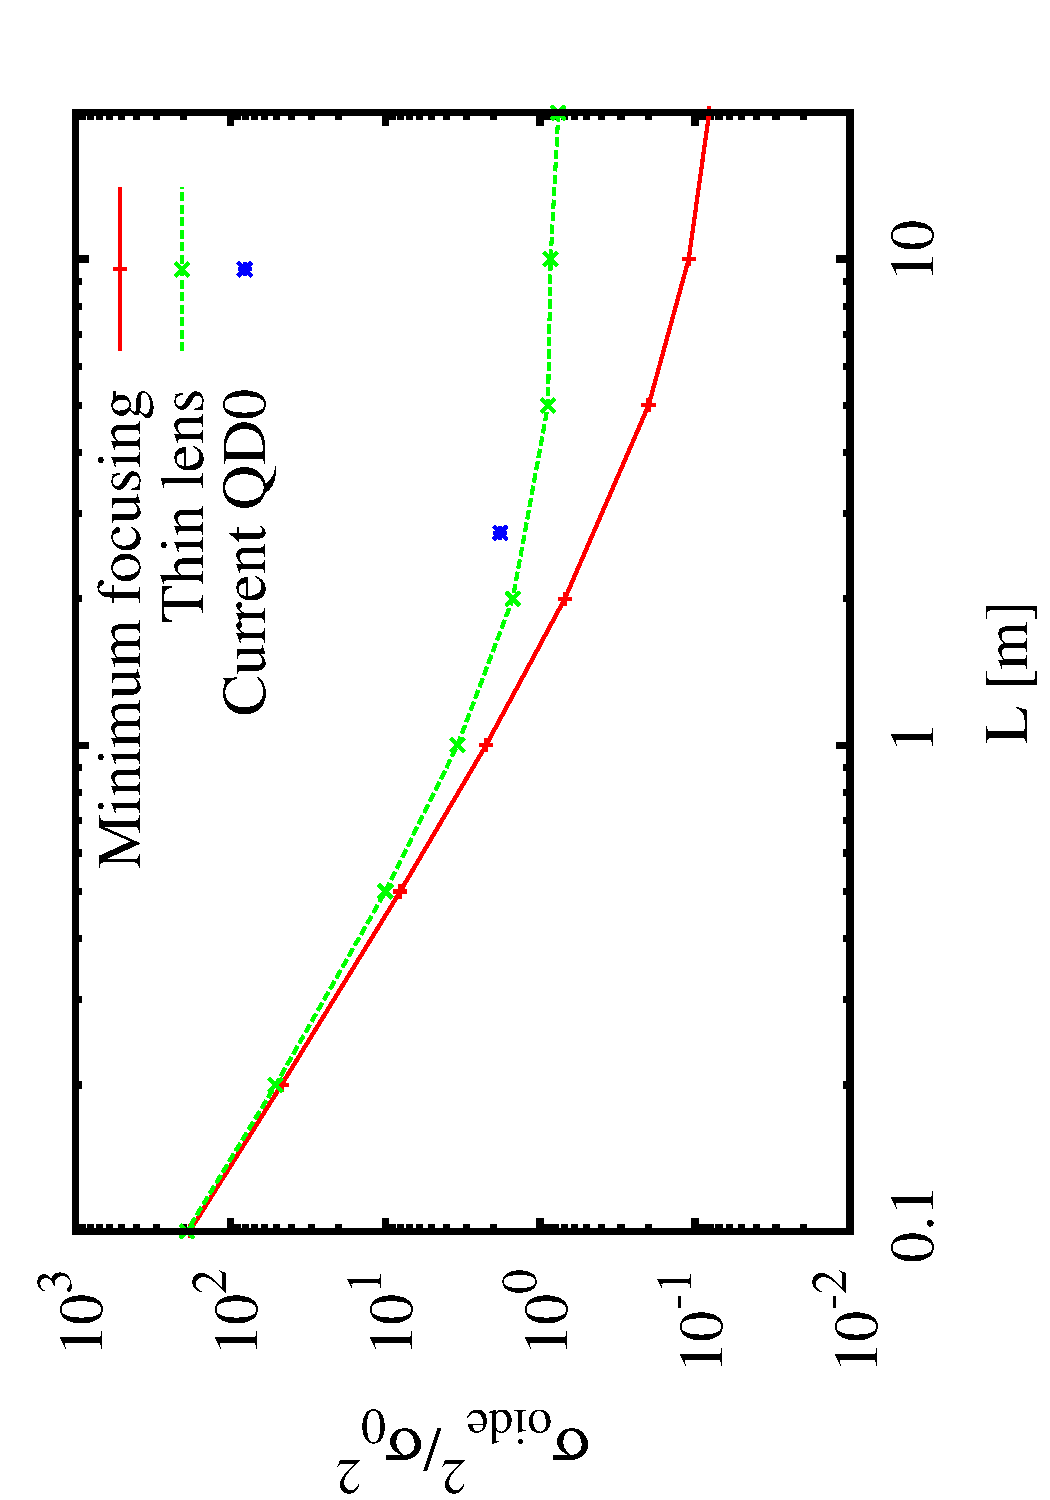
\includegraphics[scale=0.3,angle=-90]{image07a.pdf}\caption{}\label{fig-3TeV:a}
\end{subfigure}
\begin{subfigure}{0.45\textwidth}
\centering
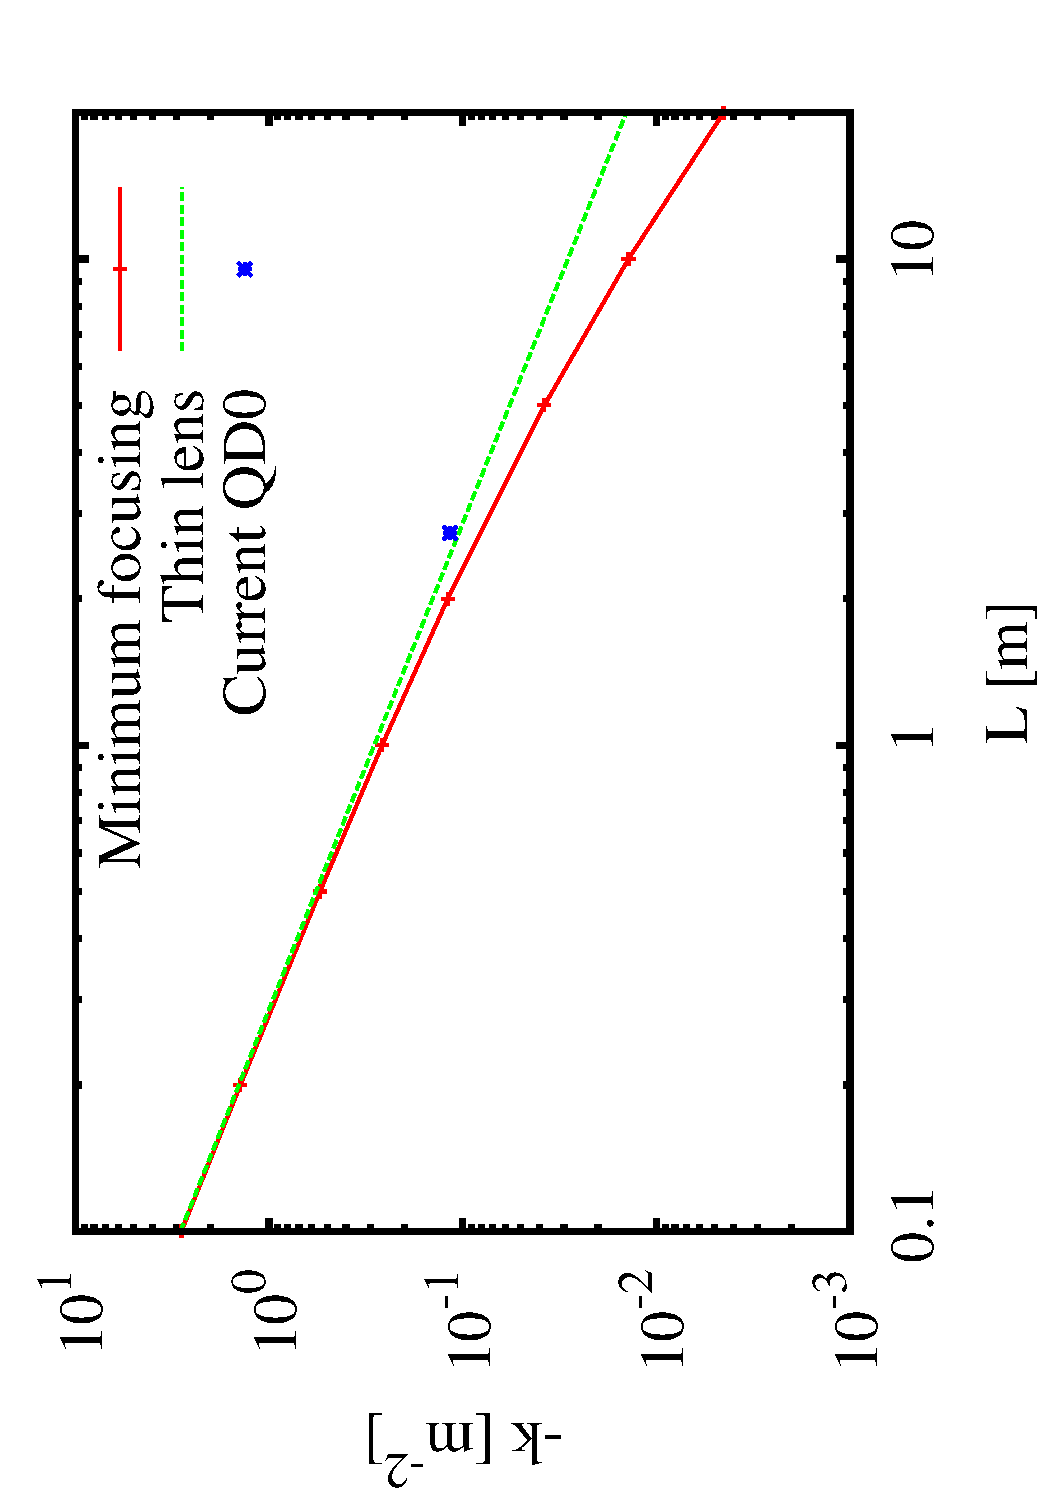
\includegraphics[scale=0.3,angle=-90]{image07b.pdf}\caption{}\label{fig-3TeV:b}
\end{subfigure}
\caption{Oide effect beam size contribution for CLIC 3 TeV design parameters. (a) $\sigma^2_{oide}$ normalized to designed linear beam size as a function of quad length for the minimum focusing $k$ (when $\alpha_y=0$ at the quadrupole opposite side to the IP), for $k$ calculated as thin lens ($k=\frac{1}{Ll^*}$) and the current QD0. (b) $k$ in the three previous cases for comparison.}\label{fig-3TeV}
 \end{figure}\par
Fig. \ref{fig-500GeV} is the corresponding to Fig. \ref{fig-3TeV} for the 500 GeV case. The current design contributes less than 4\% of the total beam size, concluding that the current QD0 length with the CLIC 500 GeV parameters does not need adjustment.\par
\begin{figure}[!htb]
\centering
\hspace*{-0.6cm}
\begin{subfigure}{0.45\textwidth}
\centering
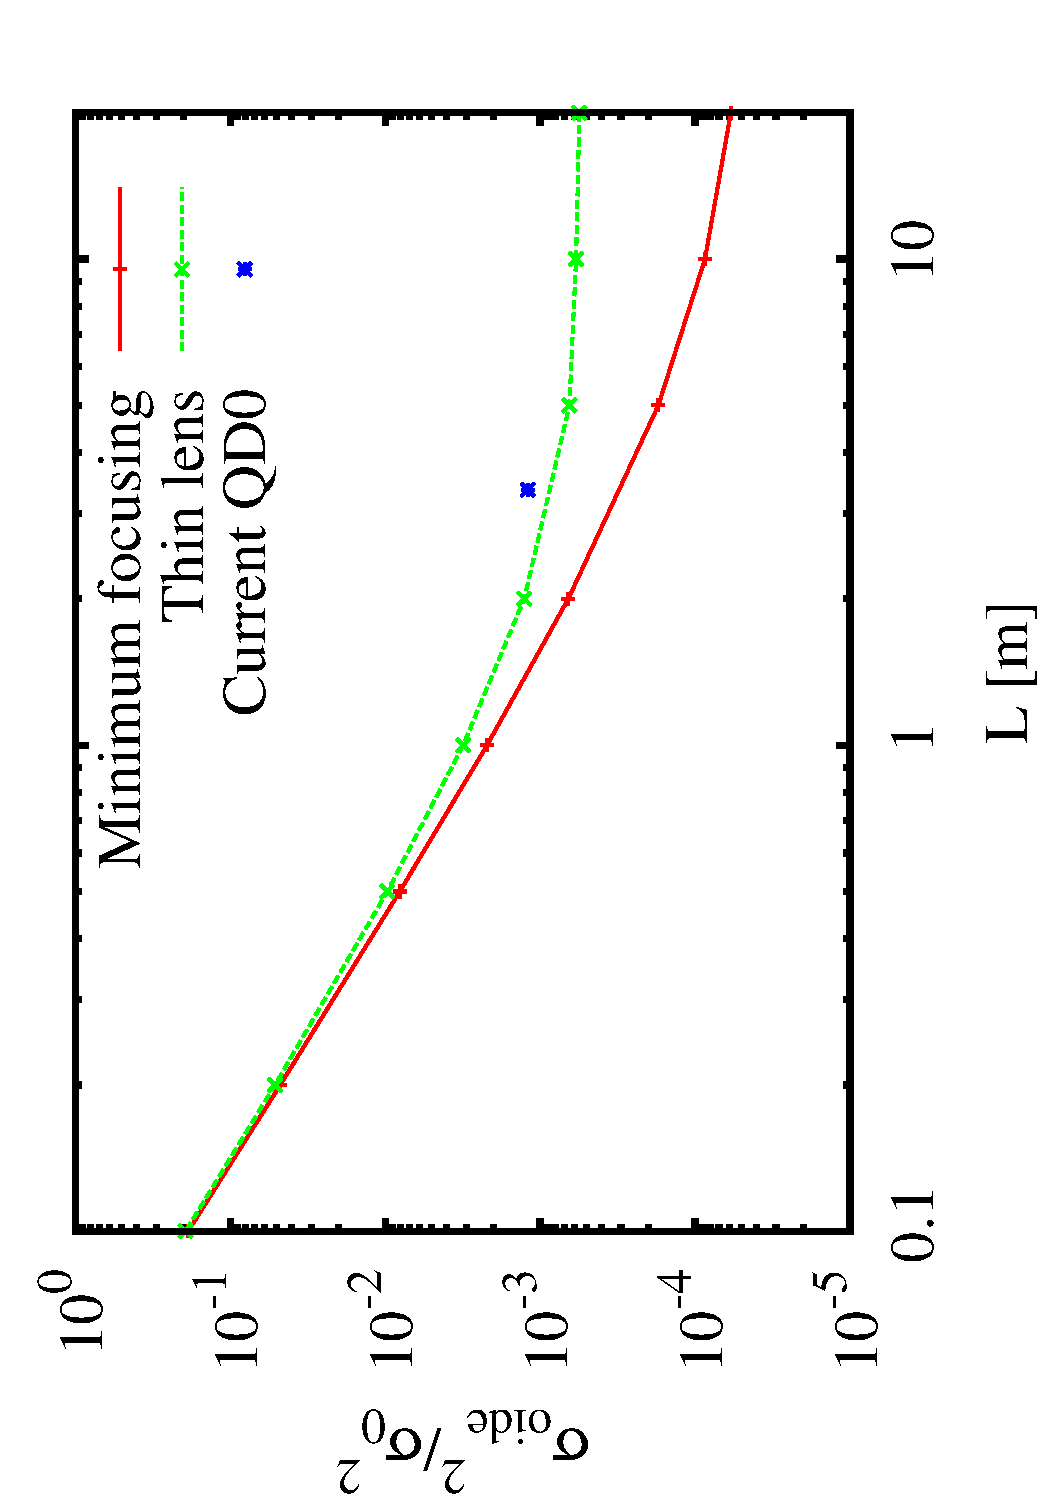
\includegraphics[scale=0.3,angle=-90]{image06b.pdf}\caption{}
\end{subfigure}
\begin{subfigure}{0.45\textwidth}
\centering
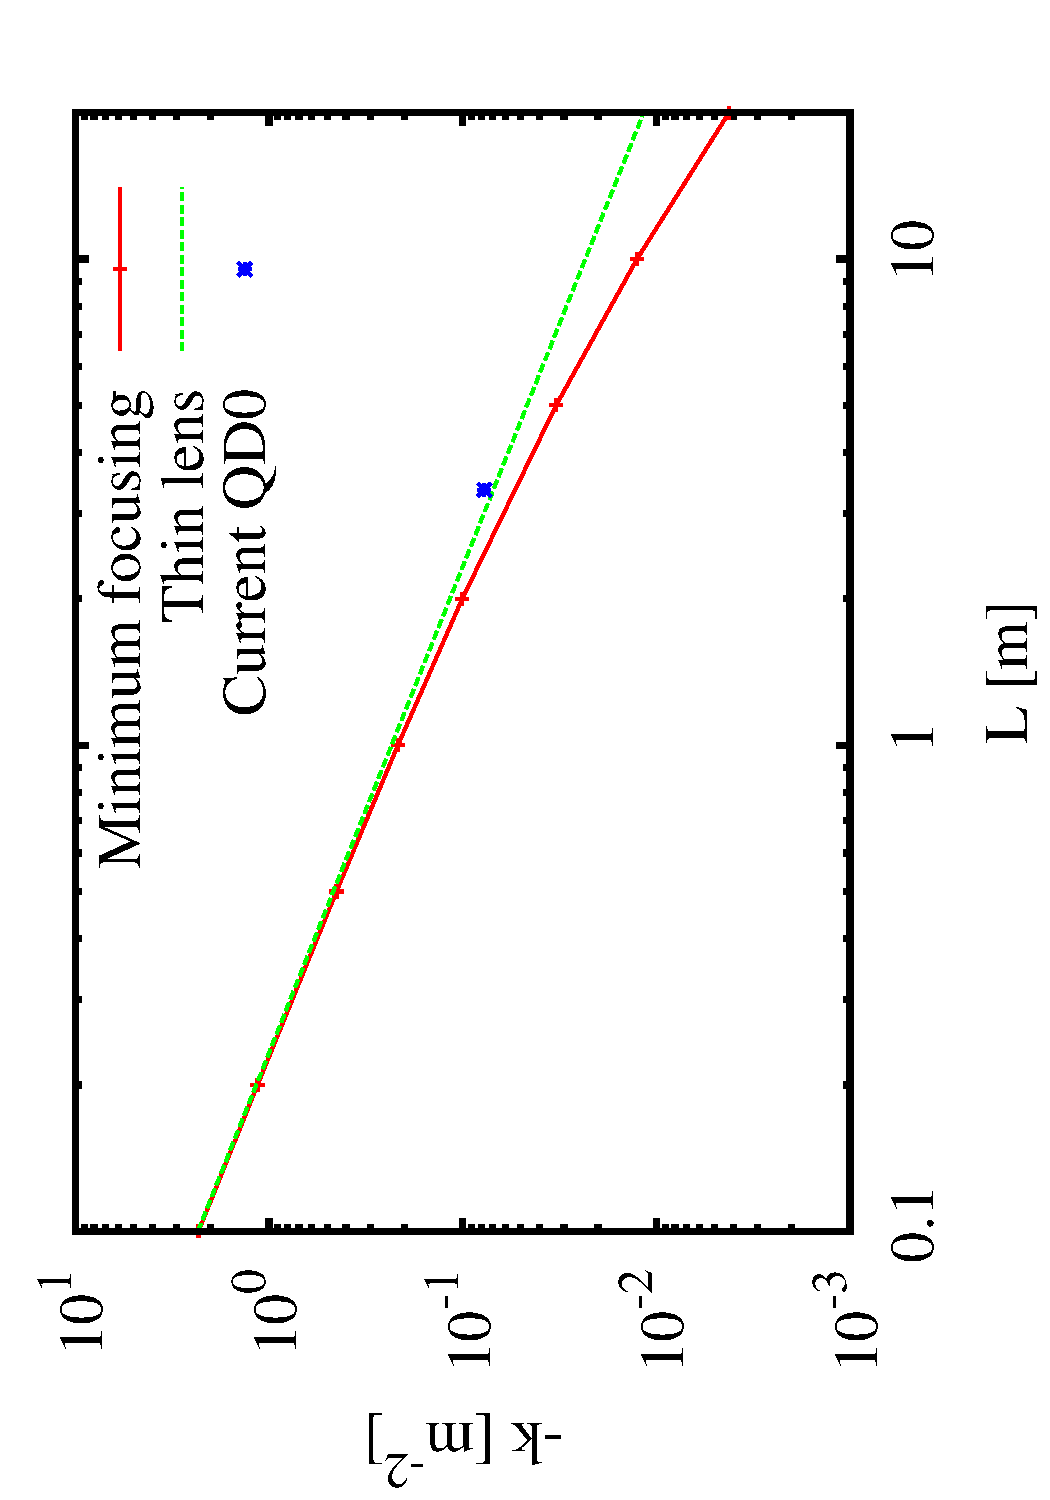
\includegraphics[scale=0.3,angle=-90]{image06c.pdf}\caption{}
\end{subfigure}
\caption{Oide effect beam size contribution for CLIC 500 GeV design parameters. (a) $\sigma^2_{oide}$ normalized to designed linear beam size as a function of quad length for the minimum focusing $k$ (when $\alpha_y=0$ at the quadrupole opposite side to the IP), for $k$ calculated as thin lens ($k=\frac{1}{Ll^*}$) and the current QD0. (b) $k$ in the three previous cases for comparison.}\label{fig-500GeV}
 \end{figure}\par

\subsection{Correctors}
\subsubsection{$\Delta y$ due to radiation}
Particle tracking from QD0 input to the IP for CLIC 3 TeV with and without radiation using PLACET \cite{Placet} gives the six dimentional phase space effect of radiation. Fig. (\ref{f:CLIC3TeVbeamsizeIP}) shows the current transversal distribution of particles. The ideal would be to remove the change due to radiation $\Delta y = y_\text{rad} -y_0$.\par
\begin{figure}[!htb]
\centering
 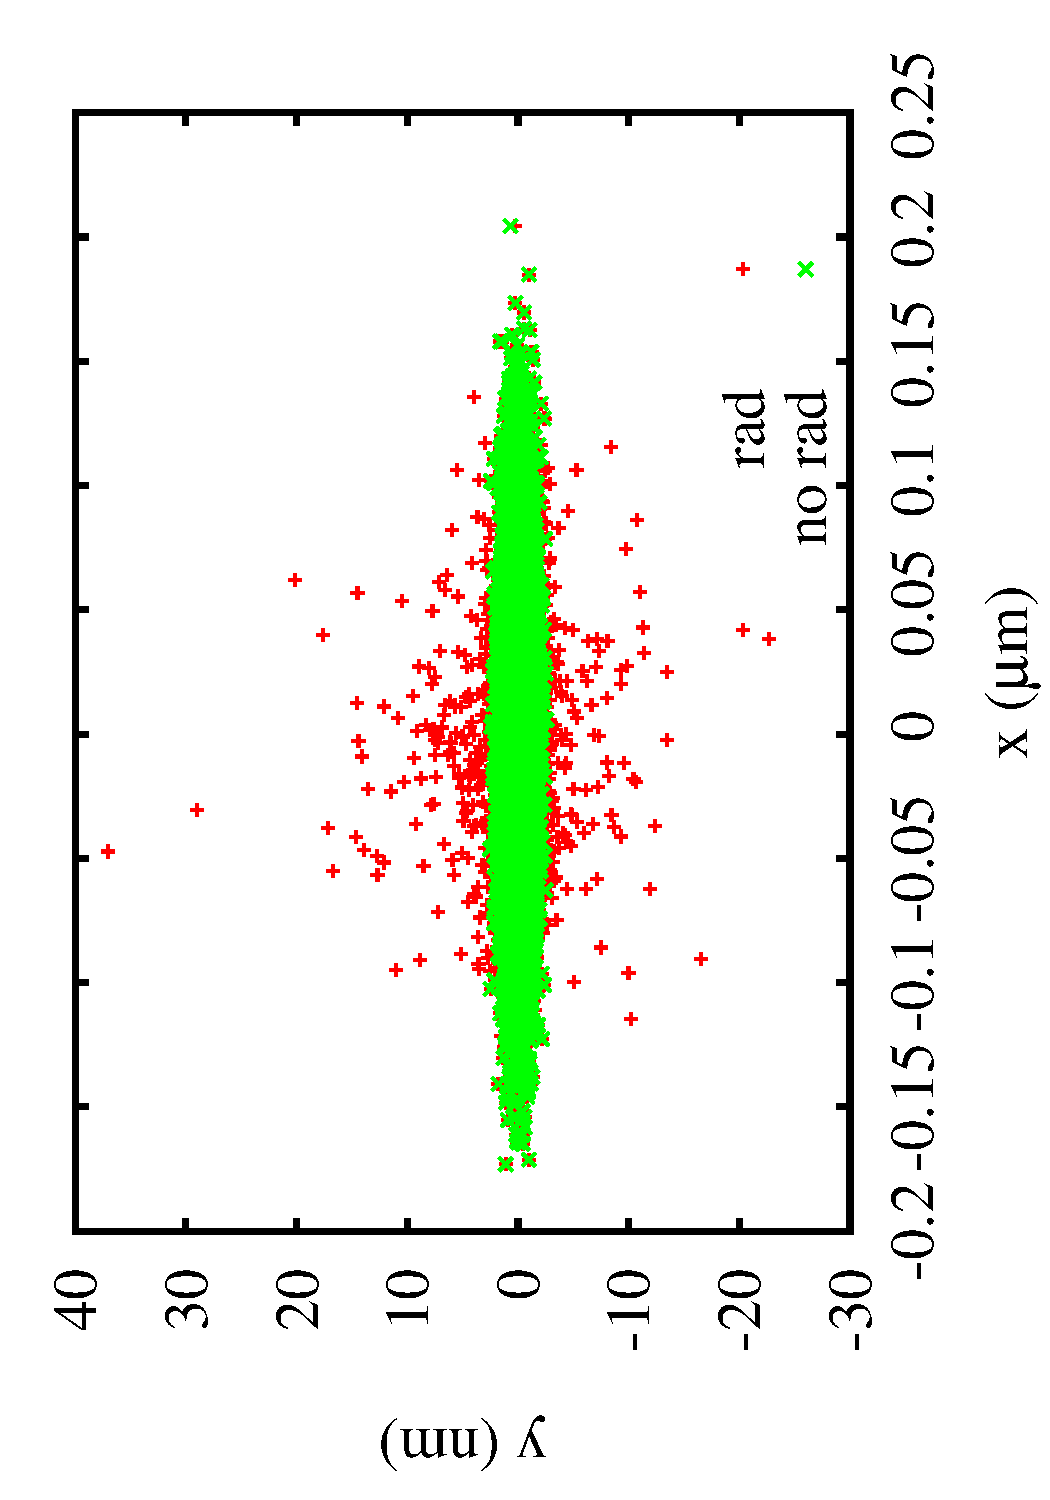
\includegraphics[scale=0.3,angle=-90]{plotxyrad.pdf}\caption{CLIC 3 TeV beam at the IP after tracking QD0 with and without radiation.}\label{f:CLIC3TeVbeamsizeIP}
\end{figure}
Although the average radiation effect is zero, $\langle \Delta y \rangle = 0$ because of the term $(y_0')^3$ as stated by Oide, the correlation between $\Delta y, y'$ is not zero. Here I show the radiation average expression as a function of $y_0'$.
\begin{equation}
 \langle\Delta y (y'_0)\rangle = \frac{2}{3}r_e\gamma^3G(\sqrt{K}L,\sqrt{K}L^*)(y'_0)^3
\end{equation}
%$r_e$ is the clasical electron radius and 
where $G(\sqrt{K}L,\sqrt{K}L^*)$ is
\begin{equation}
\int_0^{\sqrt{K}L}(\sin\phi+\sqrt{K}L^*\cos\phi)^2\int_0^\phi (\sin\phi'+\sqrt{K}L^*\cos\phi')^2 d\phi'd\phi
\end{equation}
Fig. (\ref{f:correlation}) shows the comparison between the correlation obtained from tracking and the theoretical evaluation of the previous expression.\par
\begin{figure}[!htb]
\centering
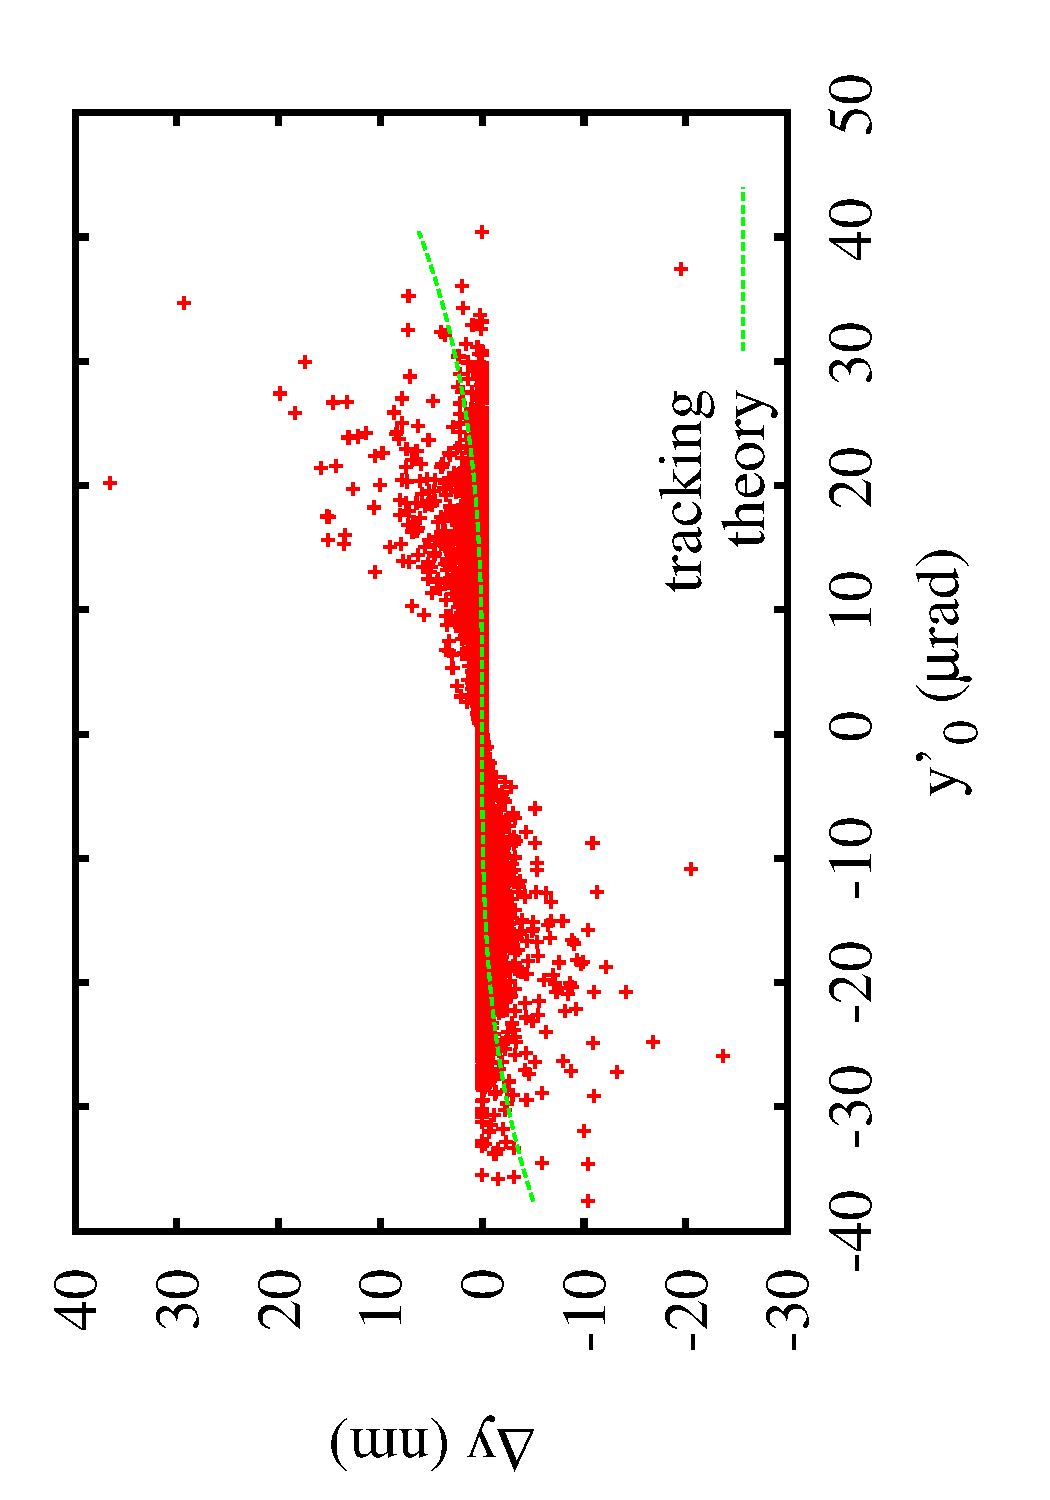
\includegraphics[scale=0.3,angle=-90]{plotdyrad.pdf}\caption{Correlation between the phase space coordinates $y,y'$ for CLIC 3 TeV from particle tracking and theoretical expression.}\label{f:correlation}
\end{figure}
This correlation could be removed from the beam size by a set of correctors to be presented in next Section.
\subsubsection{Correctors}
A pair of correctors, as in Fig. (\ref{f:corrector}), is added to the strong focusing in order to mitigate the radiation effect. The procedure consists in scan the best position and multipole gradient ($s,k_i$) for C0, and then set C1 at QD0 input to cancel the effect of C0.\par
\begin{figure}[!htb]
\centering
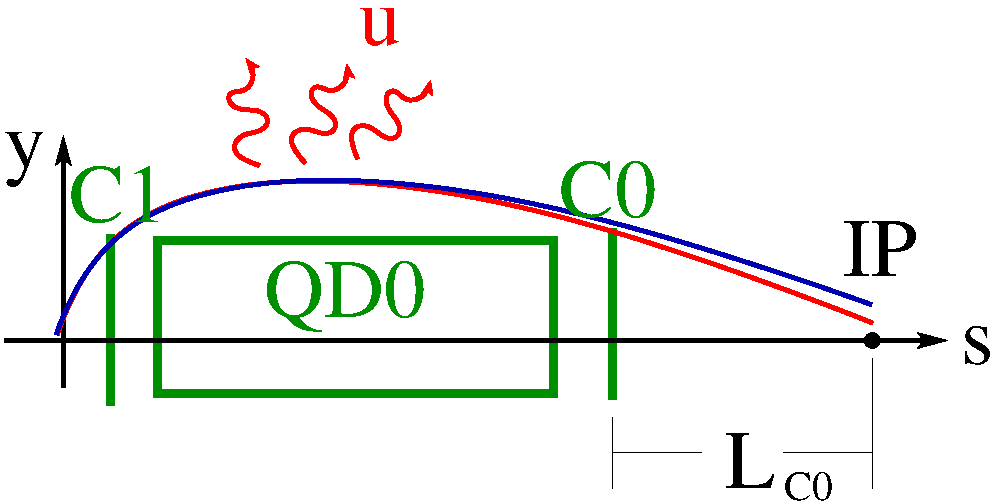
\includegraphics[scale=0.3,angle=0]{Oide2.pdf}\caption{For the nominal trajectory in blue, the kick in C1 must cancel the kick in C0. For all particles that radiate in red, the difference in kicks should cancel $\Delta y$.}\label{f:corrector}
\end{figure}
Two sets of correctors (C0,C1) where tried. Quadrupoles (QD00,QD01) to substract the equivalent of a linear fit, and Octupoles (OD0,OD1) for a cubic fit.
\begin{table}[!hbt]
\centering
\begin{tabular}{l||c|c|c}\hline\hline
Corrector & i & $L$ & $k_{i}$\\
& & (m)& (m$^{-(i+1)}$)\\\hline
QD00 & 1 & 0.01 &\\
QD01 & 1 & 0.01 &\\\hline
OD0 & 3 & 0.01 & 36\\
OD1 & 3 & 0.01 & 0\\\hline
\end{tabular}\caption{Correctors}\label{t:correctors}
\end{table}

\subsubsection{Beam size and luminosity results }

\subsubsection{Limitations}
It was not possible to reduce the correlation more because even that C0 adds very little to radiation. But at some point the radiation in C1 starts to be important. It might be possible to scan  C1 ($s,k$) to find a place where it radiates less. Even with perfect C1 to C0 correction there will be a limit when radiation will affect the Horizontal plane. Here the target was set to less than 1\% of horizontal beam size increase. Mean correlation could be reduced to a minimum as there is not correlation per each particle... (other target?)

\section{Conclusions}
Radiation in the final quad sets a limit on the vertical beamsize, this is called Oide effect. Even if the mean value of the trajectory change is zero, there is a correlation between the change in trajectory and the angle at the IP due to the energy change. This correlation is reduced by correctors before and after QD0. The best result yet has been with octupoles giving a vertical beam size reduction of $(4.3\pm??)$\%
